\chapter{Konzeption}
\label{chapter4}
Vor der eigentlichen Implementierung erfolgt nun die Konzeption.
Damit wird elaboriert, welche Anforderungen an die Software gestellt werden
und wie die Implementierung erfolgen muss.
Etwaige Ungereimtheiten und Probleme können so frühzeitig erkannt werden.

\section{Anforderungsanalyse}
\label{4-Anforderungsanalyse}
Es soll ein System implementiert werden,
welches Kinect-Bewegungsdaten mithilfe von hierarchischem Clustering
und \ac{DTW} als Distanzmetrik gruppiert.
Dieses Tool kann im Rahmen des HoPE-Projekts genutzt werden,
um große Datensätze auf wiederkehrende Bewegungsabläufe bei der Interaktion mit Wandbildschirmen
hin zu untersuchen.
Es gibt sogenannte \emph{funktionale Anforderungen} und \emph{nicht-funktionale Anforderungen},
die das System erfüllen muss.
Letztere beinhalten beispielsweise Anforderungen zu Benutzbarkeit, Effizienz oder Portierbarkeit.
Funktionale Anforderungen beschreiben hingegen die primären Funktionen des Systems.

\subsection{Nicht-funktionale Anforderungen}
\label{4-NichtFunktionaleAnforderungen}
Bei der Wahl der Programmiersprache und möglichen verwendeten Frameworks
existieren keine speziellen Vorgaben.
Das Tool soll allerdings ohne großen Installationsaufwand nutzbar sein
und daher nach Möglichkeit eine stark verbreitete Programmiersprache nutzen.
Bei der Implementierung fällt daher die Wahl auf Java in der Version 14.
Dabei sollen auch keine externen Bibliotheken genutzt werden.
An die Effizienz gibt es ebenfalls keine besonderen Anforderungen,
da die Auswertung der Daten nur einmalig erfolgt.
Eine Echtzeitauswertung ist nicht geplant.
Da zu lange Wartezeiten, aber die Nutzbarkeit des Tools einschränken,
sollen berechnete Kosten in einer geeigneten Datenstruktur zwischengespeichert werden.
So können im darauffolgenden Iterationsschritt Berechnungsschritte eingespart werden.
Das Tool soll durch wenige Anpassungen auch auf Datensätze anderer Tiefenkameras angewandt werden können.
Um dieses Ziel zu erreichen, wird die Software von Beginn an generisch entwickelt.
Zu allen Bestandteilen des Tools existiert daher ein Interface.
Bei Bedarf können so einfach neue Implementierungen,
die den Anforderungen anderer Datensätze entsprechen, ergänzt werden.

\subsection{Funktionale Anforderungen}
\label{4-FunktionaleAnforderungen}
Die Anwendung sollte die folgenden Funktionalitäten anbieten.
Unter anderem kümmert sie sich um den Input.
Ein Datensatz kann aus Textdateien eingelesen und in passenden Datenobjekten abgespeichert werden.
Das Tool soll ein Clustering mittels hierarchischem Clustering wie in \autoref{3-Clustering} beschrieben anbieten.
Dabei ist der Threshold für das Mergen von zwei Clustern vom Nutzer konfigurierbar.
Als Distanzmetrik wird \ac{DTW} (\autoref{3-DTW}) genutzt.
Dabei ist konfigurierbar, welche Attribute des Datensatzes für den Vergleich genutzt werden.
Zur Berechnung der Distanz zwischen zwei Punkten wird die euklidische Distanz verwendet.
Allerdings können hier weitere Funktionen ergänzt werden.
Mit Hilfe eines Startparameters kann entschieden werden, welche dieser Funktionen für die Berechnung verwendet wird.
Zudem besitzt das Tool Output-Funktionalitäten.
Die gefundenen Cluster werden in einer Textdatei aufgelistet.
Jedes Cluster erhält eine eindeutige Identifikationsnummer und eine Liste aller Records die zusammengeführt wurden.
Für ein erleichtertes Verständnis der Cluster wird auch eine primitive Visualisierung der Cluster angeboten.
Die starke Konfigurierbarkeit wird durch eine \emph{config-file} erreicht,
die der Nutzer beim Start der Anwendung übergeben kann.
\autoref{tbl:AttributesConfig} zeigt deren Attribute.
\begin{table}[ht]
    \begin{center}
        \begin{tabular}{ |c|c| } 
            \hline
            Attributname & Beschreibung \\
            \hline \hline
            inputPath & Pfad zum Datensatz. \\
            \hline
            outputPath & Pfad zum Ablegen der Output-Dateien.  \\
            \hline
            separator & Trennzeichen zwischen den Attributen. \\
            \hline
            datasetType & Art des vorliegenden Datensatzes. \\
            \hline
            threshold & Grenzwert für das Zusammenführen von Clustern. \\
            \hline
            attributes & Vorhandene Attribute. \\
            \hline
            usedAttributes & Attribute, die zum Vergleich genutzt werden. \\
            \hline
            distanceFunction & Bezeichnung der genutzten Distanzfunktion. \\
            \hline
            flipVisualization & Wahrheitswert, ob die Visualisierung gespiegelt wird. \\
            \hline
            attributeForBodyIdentification & Bezeichnung des Körperidentifikationsparameters. \\
            \hline
            skipFrames & Wahrheitswert, ob jeder zweite Frame ignoriert wird. \\
            \hline
        \end{tabular}
        \caption{Attribute der Configuration-Datei.}
        \label{tbl:AttributesConfig}
    \end{center}
\end{table}

\clearpage
\section{Programmablauf}
\label{4-Programmablauf}
Im Folgenden wird der Programmablauf beschrieben.
\begin{enumerate}
    \item Der Nutzer startet den \emph{Clustering-Processor}
    und gibt als Startparameter den Pfad der \emph{config-Datei} an.
    \item Der \emph{Processor} nutzt den \emph{Config-Reader}, um die Werte der \emph{Konfigurationdatei} auszulesen
    und speichert diese ab.
    \item Der \emph{Processor} nutzt den \emph{DataReader}, um den Datensatz einzulesen
    und legt die Informationen in geeigneten Objekten ab.
    Beim Kinect-Datensatz sind das die Implementierungen \emph{RecordImpl} und \emph{FrameImpl}
    der entsprechenden Interfaces.
    \item Der \emph{Processor} startet das Clustering durch den Aufruf der \emph{cluster-Methode}
    eines \emph{HierarchicalClustering-Objekts}.
    Zu beginn entspricht jeder Record einem eigenen Cluster.
    Die \emph{recordToCluster-Methode} ermöglicht eine Transformation.
    \item Das Clustering nutzt ein \emph{\ac{DTW}-Objekt},
    um paarweise die Kosten zweier Cluster zu berechnen.
    \item Die beiden Cluster mit den geringsten Kosten werden zusammengeführt.
    Konkret wird eines der Cluster in das andere integriert.
    Dadurch entsteht eine Kombination beider Cluster.
    Beim integrierten wird ein boolescher Wert auf \emph{false} gesetzt,
    damit das Cluster in späteren Berechnungsschritten nicht mehr beachtet wird.
    Dabei wird jeweils das Mittel der Attributwerte berechnet und abgelegt.
    Zudem werden die Cluster-Bestandteile abgespeichert.
    Bei allen Komponenten wird ebenfalls der boolesche Wert auf \emph{false} gesetzt,
    damit sie bei zukünftigen Vergleichen nicht mehr berücksichtigt werden.
    \item Schritte 5 und 6 werden so lange wiederholt, bis die geringsten Kosten den vom Nutzer definierten Threshold übersteigen.
    \item Der \emph{Processor} nutzt den \emph{Cluster-Writer}, um alle Cluster der \emph{clusters-Liste}
    in eine Ausgabedatei zu schreiben.
    \item Der \emph{Processor} nutzt die \emph{VisualizerImpl}, um alle Records der gefundenen Cluster zu visualisieren.
    \item Die Anwendung terminiert. 
\end{enumerate}

\section{Teilsysteme}
\label{4-Teilsysteme}
\autoref{fig:Packages} kann das Paketdiagramm des Tools entnommen werden.
Das Paket \emph{model} enthält die Interfaces für Cluster, Records und Frames.
Außerdem jeweils geeignete Implementierungen dieser Interfaces für den Kinect-Datensatz.
Bei Bedarf können hier bei späterer Verwendung der Software weitere Implementierungen
für andere Datensätze ergänzt werden.
Im \emph{utility}-Paket befinden sich Interfaces für Reader und Writer.
Auch hier sind geeignete Implementierungen bereitgestellt.
Konkret ein Reader für die Config-Datei, ein Reader für die Kinect-Daten
und ein Writer für die gefundenen Cluster.
Auch das Interface und die Implementierung für die Visualisierung befinden sich hier.
Im Paket \emph{calculating} befindet sich alles was für das Clustern der Daten benötigt wird.
Es ist weiter untergliedert in \emph{clustering} und \emph{metric}.
Letzteres liefert die Vergleichsmetrik für unser Clusterverfahren.
Wieder liegen geeignete Interfaces vor,
sodass die Anwendung bei Bedarf um weitere Metriken oder Clustering-Ansätze erweitert werden kann.
Bereitsgestellt werden initial eine Implementierung mit hierarchischem Clustering
und \ac{DTW} als Metrik.
Das Paket \emph{processor} ist von zentraler Bedeutung.
Hier wird die Funktionalität des Tools zusammengeführt.
Zunächst werden die benötigten Reader Instanzen initialisiert.
Mit ihnen werden die Daten eingelesen.
Anschließend wird das Clustering gestartet.
Die Ergebnisse werden geeignet in der Ausgabedatei gespeichert und visualisiert.
\begin{figure}[ht]
    \begin{center}
    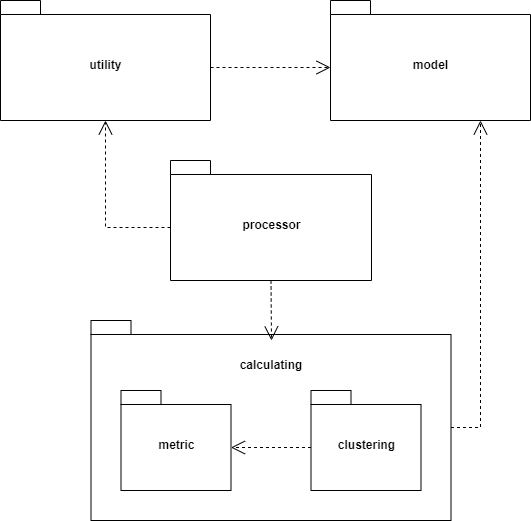
\includegraphics[width=0.9\textwidth]{packages.png}
    \end{center}
    \caption{Paketdiagramm des Tools.}
    \label{fig:Packages}
\end{figure}